\chapter{EquiDiff: Equivariant Diffusion Sampling for Invariant Set Generation}\label{r:method}

This chapter presents the theoretical foundation and algorithmic details of our proposed approach for generating invariant sets of neural network representations. We begin with formal mathematical definitions, establish the relationship to classical level sets from differential topology \citep{lee2013smooth,milnor1965topology,fort2017gaussian}, detail our core algorithm, and conclude with implementation specifics and quality assurance measures.

\section{Theoretical Foundation and Formal Definitions}

We begin by establishing the mathematical foundations for our approach through formal definitions that clarify the key concepts and their relationships.

\begin{defi}[Invariant Framework]\label{def:invariants_framework}
Let $f: \mathbb{R}^n \rightarrow \mathbb{R}^m$ be a neural network with $n$ input dimensions and $m$ output dimensions, where $n$ represents the dimensionality of the input space (e.g., $n = W \times H \times C$ for images of width $W$, height $H$, and $C$ channels) and $m$ represents the dimensionality of the network component we wish to analyze (e.g., $m = 1$ for a single neuron, $m = k$ for $k$ class logits). The network $f$ can be viewed as a composition of functions $f = f_L \circ f_{L-1} \circ \ldots \circ f_1$, where each $f_i$ represents a layer transformation.

For a given query point $\mathbf{x}^* \in \mathbb{R}^n$, the \textbf{Invariant Framework} defines the theoretical foundation for identifying all inputs that produce identical network responses under a specified objective function.
\end{defi}

\begin{defi}[EquiDiff Method]\label{def:equidiff_method}
Given the Invariant Framework (Definition \ref{def:invariants_framework}), we define the \textbf{EquiDiff method} as an algorithmic approach that combines score-based diffusion models with iterative optimization to generate diverse, realistic samples from invariant sets.

Specifically, for a neural network $f: \mathbb{R}^n \rightarrow \mathbb{R}^m$ and query point $\mathbf{x}^*$, EquiDiff generates samples $\{\mathbf{x}_i\}_{i=1}^N$ such that:
\begin{enumerate}
\item \textbf{Invariance constraint}: $\|f(\mathbf{x}_i) - f(\mathbf{x}^*)\|_2 < \epsilon$ for small $\epsilon > 0$
\item \textbf{Realism constraint}: $\mathbf{x}_i$ lies within the natural image manifold as defined by a pre-trained diffusion model
\item \textbf{Diversity constraint}: The generated samples exhibit semantic and visual diversity while maintaining the invariance constraint
\end{enumerate}

The method operates through infinite optimization over the latent space of a diffusion model, enabling precise control over network activations while ensuring realistic image generation.
\end{defi}

\begin{figure}[h]
\centering
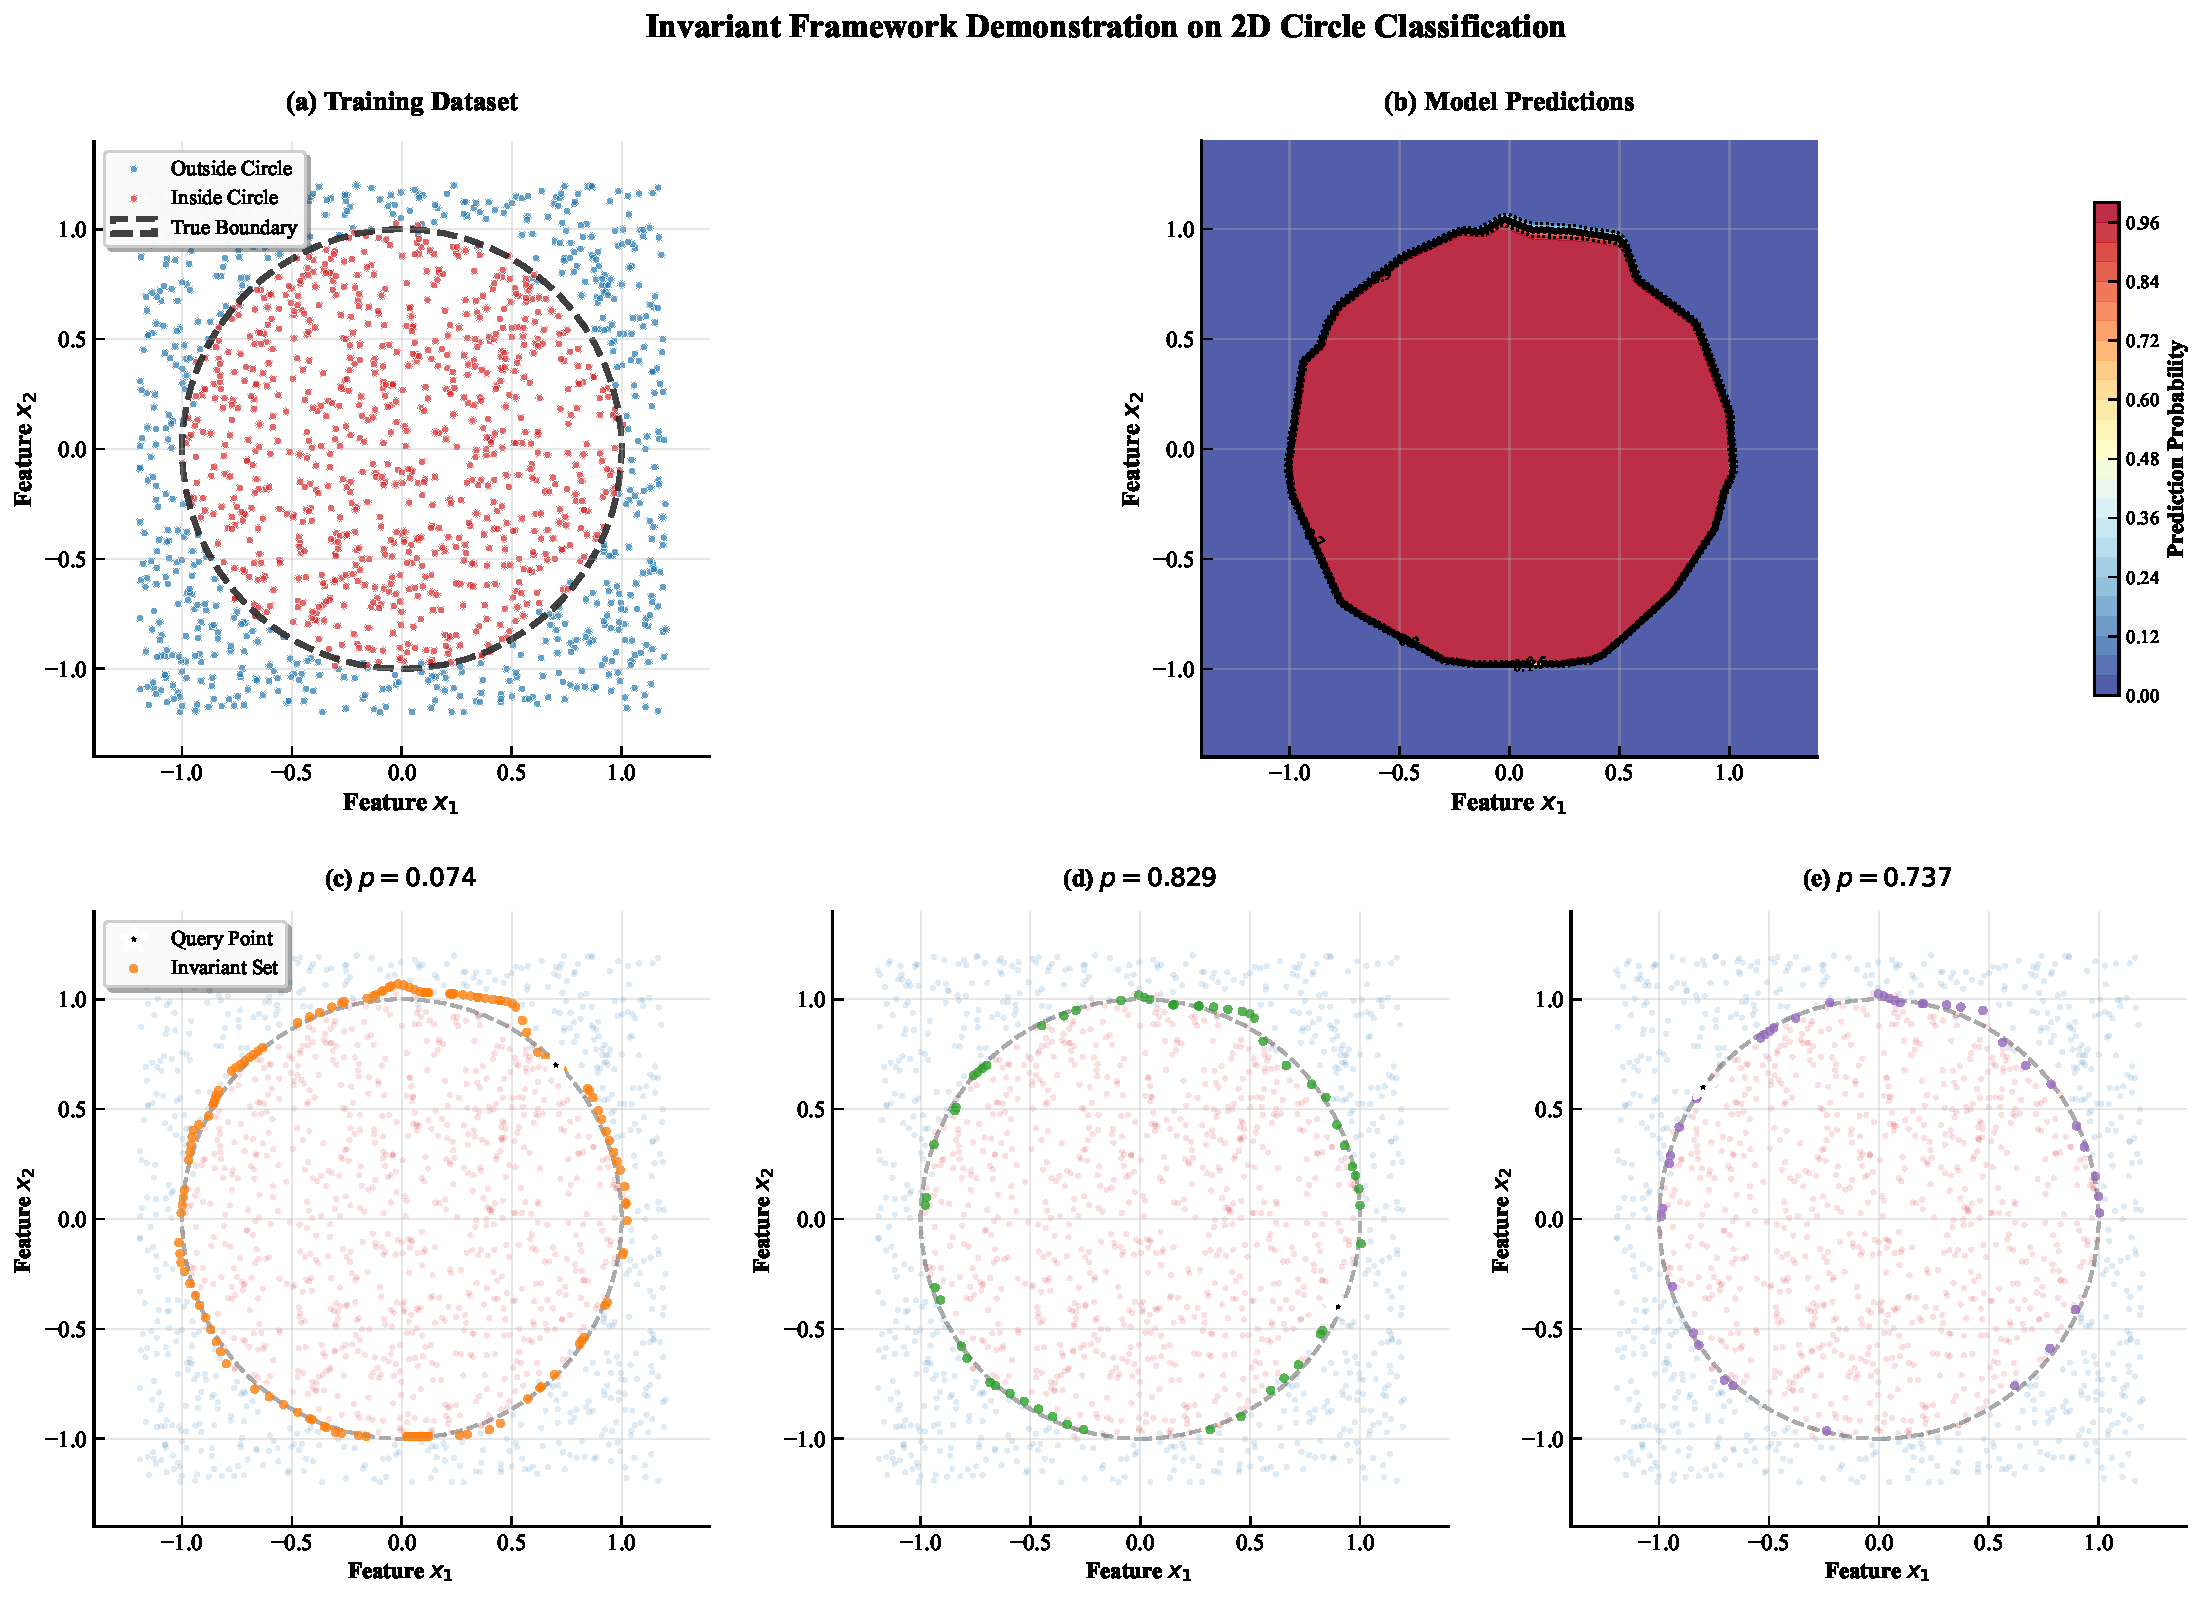
\includegraphics[width=\linewidth]{figures/main/invariant_framework_combined.pdf}
\caption{Demonstration of the Invariant Framework on a 2D Concentric Circles Dataset.
(a) Training dataset with 1,500 samples classified by their position relative to a unit circle (dashed line). Blue points represent the outer class, pink points the inner class.
(b) Learned decision boundary and prediction probability heatmap from a 3-layer MLP (test accuracy: 0.983). The black contour shows the 0.5 decision boundary.
(c-e) Invariant sets for three query points (black stars) with prediction values p. Orange points represent all input locations that yield identical predictions under the trained model, demonstrating the equivalence relation established by the model's output. The invariant sets approximate level curves of the learned decision function, revealing the geometric structure of the model's decision space.}
\label{fig:teaser}
\end{figure}

\section{Problem Formulation}
The problem of finding invariant sets (IS) is formulated as discovering members of an equivalence relation. Given a neural network with parameters $\boldsymbol{\theta}$ and objective function $\mathcal{L}_{\boldsymbol{\theta}}:\mathbb{R}^n \rightarrow \mathbb{R}^m$, and a query point $\mathbf{x^*}$, the invariant set is defined as:
\begin{equation}
  \mathbf{IS}(\mathbf{x^*}) = \{ \mathbf{x} \in \mathbb{R}^n : \mathcal{L}_{\boldsymbol{\theta}}(\mathbf{x}) = \mathcal{L}_{\boldsymbol{\theta}}(\mathbf{x^*}) \}
  \label{eq:is}
\end{equation}
We use the notation $\mathbf{x^*} \sim_{\mathcal{L}_{\boldsymbol{\theta}}} \mathbf{x}$ to denote that two elements $\mathbf{x^*}$ and $\mathbf{x}$ belong to the same invariant set under the equivalence relation defined by $\mathcal{L}_{\boldsymbol{\theta}}$.

The objective function $\mathcal{L}_{\boldsymbol{\theta}}$ can represent various neural network components: a single neuron's activation, class logits for one or multiple classes, or any differentiable function for which gradients can be computed. While adversarial examples can be viewed as specific perturbations that may belong to invariant sets under certain conditions \citep{szegedy2014intriguingpropertiesneuralnetworks}, the goal of this work is fundamentally different: one seeks to sample from the intersection of the invariant set with the natural data manifold, ensuring realism by construction.

To achieve this, this work utilizes a trained diffusion model, specifically LightningDIT \citep{yao2025vavae} \citep{yao2024fasterdit}, which excels at generating high-quality images while maintaining the mathematical constraints of invariant set membership. The diversity of examples emerges naturally from exploring different regions of this manifold intersection.


\section{Guided Iterative Optimization with Latent Diffusion Models}

Proposed algorithm integrates signals from the neural network function $f_{\boldsymbol{\theta}}:\mathbb{R}^{W \times H} \rightarrow \mathbb{R}^m$ through a scalar loss function $\ell: \mathbb{R}^m \times \mathbb{R}^m \rightarrow \mathbb{R}$ to conditionally synthesize images from invariant sets. Given a target output $\mathbf{y^*} = f_{\boldsymbol{\theta}}(\mathbf{x^*})$, the objective is defined as:
\begin{equation}
\mathcal{L}(\mathbf{x}) = \ell(f_{\boldsymbol{\theta}}(\mathbf{x}), \mathbf{y^*})
\end{equation}
where $\ell$ is typically the $\ell_2$ norm or another appropriate distance metric. This formulation enables gradient computation for optimization while maintaining the invariant set constraint $\mathcal{L}(\mathbf{x}) = 0$. There are two primary approaches for conditioning generation using this objective.

\subsection{Classifier Guidance Limitations}

Classifier Guidance (CG) \citep{dhariwal2021diffusionmodelsbeatgans} offers a simple, computationally efficient method for trading diversity for fidelity using gradients from the objective function at each denoising step. However, this work identified two significant limitations that limit its applicability to invariant set generation.

The first limitation concerns the restrictive optimization horizon inherent in the classifier guidance approach. CG typically constrains optimization to a single forward pass through the diffusion steps, which proves too restrictive for achieving optimal results in invariant set generation. While iterative refinement through multiple passes remains theoretically possible, such approaches significantly increase computational overhead and may not converge to the precise activation values required for invariant set membership.

The second limitation involves latent space complications that arise from architectural choices in modern diffusion models. Contemporary diffusion models often employ the Latent Diffusion Model (LDM) approach \citep{rombach2022highresolutionimagesynthesislatent}, which operates in a compressed latent space rather than directly on pixel values. This architectural choice introduces additional complexity when conditioning on neural network outputs, as the classifier must evaluate encoded representations $\mathcal{E}(\mathbf{x}_t)$ at intermediate diffusion timesteps rather than natural images. This fundamental mismatch between the diffusion model's latent space and the classifier's expected input domain requires either training timestep-specific classifiers or using approximate reconstructions $\hat{\mathbf{x}}_0(t)$, both approaches introducing additional sources of error that compound throughout the generation process.

\subsection{Infinite Optimization Approach}

Given these limitations, this work adopts an \textit{Infinite Optimization} strategy, specifically adapting Algorithm~1 from \citep{augustin2024digindiffusionguidanceinvestigating}. This approach decouples the optimization process from the diffusion sampling steps, allowing for more flexible and thorough exploration of the invariant set while maintaining image quality and realism. The detailed algorithm specification is provided in \cref{appendix:infinite_optimization}.

\section{Quality and Realism Assurance}\label{method:quality_realism}

Proposed approach ensures that generated images maintain high quality and realism through several mechanisms. This work builds upon state-of-the-art frameworks for synthetic image detection and leverages the inherent properties of diffusion models, which naturally generate samples from the learned data distribution. Unlike optimization-based adversarial methods that may introduce imperceptible high-frequency artifacts, proposed diffusion-based approach constrains generation to the natural image manifold, ensuring that invariant set samples remain visually coherent and realistic.

\subsection{Frequency Domain Optimization}

To address potential high-frequency artifacts, this work performs frequency domain optimization that guides the generation process to encode meaningful signals in low-frequency bands---those visible to the human eye. Specifically, this work introduces a low-pass filter $\mathcal{F}$ before the objective function $\mathcal{L}$ and measures deviation from the original measurement across different cutoff frequencies $f_c$.

This frequency-aware approach ensures that:
\begin{itemize}
  \item Generated images appear natural to human observers
  \item Invariant set membership is achieved through semantically meaningful variations rather than imperceptible noise
  \item The generated samples maintain the visual characteristics expected from the underlying data distribution
\end{itemize}

The combination of infinite optimization with frequency domain constraints allows proposed method to generate diverse, high-quality samples from invariant sets while preserving both mathematical rigor and visual realism.
